% Created by tikzDevice version 0.12.3.1 on 2022-09-19 22:27:55
% !TEX encoding = UTF-8 Unicode
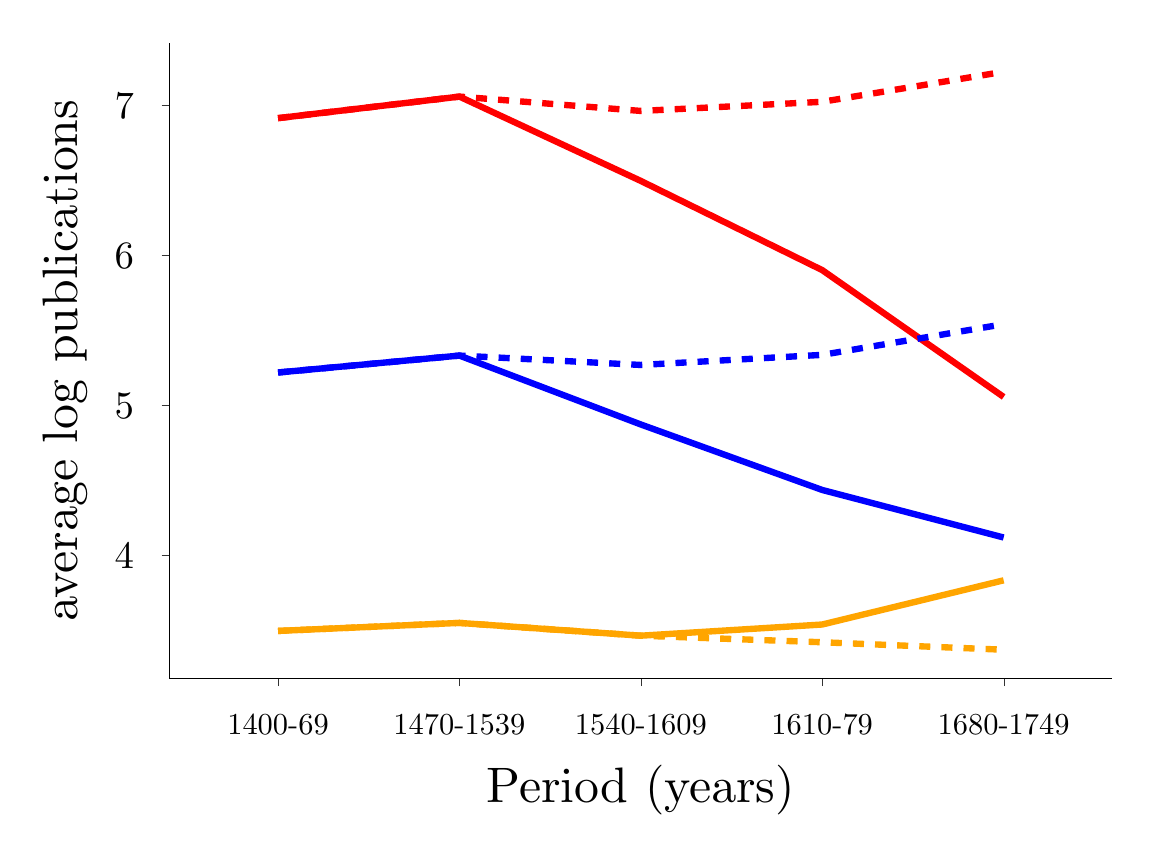
\begin{tikzpicture}[x=1pt,y=1pt]
\definecolor{fillColor}{RGB}{255,255,255}
\path[use as bounding box,fill=fillColor,fill opacity=0.00] (0,0) rectangle (397.48,289.08);
\begin{scope}
\path[clip] (  0.00,  0.00) rectangle (397.48,289.08);
\definecolor{drawColor}{RGB}{255,255,255}
\definecolor{fillColor}{RGB}{255,255,255}

\path[draw=drawColor,line width= 0.1pt,line join=round,line cap=round,fill=fillColor] (  0.00,  0.00) rectangle (397.48,289.08);
\end{scope}
\begin{scope}
\path[clip] ( 51.14, 53.86) rectangle (391.98,283.58);
\definecolor{fillColor}{RGB}{255,255,255}

\path[fill=fillColor] ( 51.14, 53.86) rectangle (391.98,283.58);
\definecolor{drawColor}{RGB}{255,0,0}

\path[draw=drawColor,line width= 2.3pt,line join=round] ( 90.47,256.38) --
	(156.02,264.17) --
	(221.56,233.70) --
	(287.11,201.47) --
	(352.66,155.64);

\path[draw=drawColor,line width= 2.3pt,dash pattern=on 4pt off 4pt ,line join=round] ( 90.47,256.38) --
	(156.02,264.17) --
	(221.56,258.99) --
	(287.11,262.29) --
	(352.66,273.14);
\definecolor{drawColor}{RGB}{0,0,255}

\path[draw=drawColor,line width= 2.3pt,line join=round] ( 90.47,164.47) --
	(156.02,170.59) --
	(221.56,145.69) --
	(287.11,122.03) --
	(352.66,104.85);

\path[draw=drawColor,line width= 2.3pt,dash pattern=on 4pt off 4pt ,line join=round] ( 90.47,164.47) --
	(156.02,170.59) --
	(221.56,167.20) --
	(287.11,170.85) --
	(352.66,181.93);
\definecolor{drawColor}{RGB}{255,165,0}

\path[draw=drawColor,line width= 2.3pt,line join=round] ( 90.47, 71.09) --
	(156.02, 73.99) --
	(221.56, 69.37) --
	(287.11, 73.41) --
	(352.66, 89.38);

\path[draw=drawColor,line width= 2.3pt,dash pattern=on 4pt off 4pt ,line join=round] ( 90.47, 71.09) --
	(156.02, 73.99) --
	(221.56, 69.37) --
	(287.11, 67.00) --
	(352.66, 64.30);
\end{scope}
\begin{scope}
\path[clip] (  0.00,  0.00) rectangle (397.48,289.08);
\definecolor{drawColor}{RGB}{0,0,0}

\path[draw=drawColor,line width= 0.1pt,line join=round] ( 51.14, 53.86) --
	( 51.14,283.58);
\end{scope}
\begin{scope}
\path[clip] (  0.00,  0.00) rectangle (397.48,289.08);
\definecolor{drawColor}{RGB}{0,0,0}

\node[text=drawColor,anchor=base east,inner sep=0pt, outer sep=0pt, scale=  1.40] at ( 38.39, 93.70) {4};

\node[text=drawColor,anchor=base east,inner sep=0pt, outer sep=0pt, scale=  1.40] at ( 38.39,147.89) {5};

\node[text=drawColor,anchor=base east,inner sep=0pt, outer sep=0pt, scale=  1.40] at ( 38.39,202.08) {6};

\node[text=drawColor,anchor=base east,inner sep=0pt, outer sep=0pt, scale=  1.40] at ( 38.39,256.27) {7};
\end{scope}
\begin{scope}
\path[clip] (  0.00,  0.00) rectangle (397.48,289.08);
\definecolor{drawColor}{gray}{0.20}

\path[draw=drawColor,line width= 0.1pt,line join=round] ( 48.39, 98.52) --
	( 51.14, 98.52);

\path[draw=drawColor,line width= 0.1pt,line join=round] ( 48.39,152.71) --
	( 51.14,152.71);

\path[draw=drawColor,line width= 0.1pt,line join=round] ( 48.39,206.90) --
	( 51.14,206.90);

\path[draw=drawColor,line width= 0.1pt,line join=round] ( 48.39,261.09) --
	( 51.14,261.09);
\end{scope}
\begin{scope}
\path[clip] (  0.00,  0.00) rectangle (397.48,289.08);
\definecolor{drawColor}{RGB}{0,0,0}

\path[draw=drawColor,line width= 0.1pt,line join=round] ( 51.14, 53.86) --
	(391.98, 53.86);
\end{scope}
\begin{scope}
\path[clip] (  0.00,  0.00) rectangle (397.48,289.08);
\definecolor{drawColor}{gray}{0.20}

\path[draw=drawColor,line width= 0.1pt,line join=round] ( 90.47, 51.11) --
	( 90.47, 53.86);

\path[draw=drawColor,line width= 0.1pt,line join=round] (156.02, 51.11) --
	(156.02, 53.86);

\path[draw=drawColor,line width= 0.1pt,line join=round] (221.56, 51.11) --
	(221.56, 53.86);

\path[draw=drawColor,line width= 0.1pt,line join=round] (287.11, 51.11) --
	(287.11, 53.86);

\path[draw=drawColor,line width= 0.1pt,line join=round] (352.66, 51.11) --
	(352.66, 53.86);
\end{scope}
\begin{scope}
\path[clip] (  0.00,  0.00) rectangle (397.48,289.08);
\definecolor{drawColor}{RGB}{0,0,0}

\node[text=drawColor,anchor=base,inner sep=0pt, outer sep=0pt, scale=  1.10] at ( 90.47, 33.53) {1400-69};

\node[text=drawColor,anchor=base,inner sep=0pt, outer sep=0pt, scale=  1.10] at (156.02, 33.53) {1470-1539};

\node[text=drawColor,anchor=base,inner sep=0pt, outer sep=0pt, scale=  1.10] at (221.56, 33.53) {1540-1609};

\node[text=drawColor,anchor=base,inner sep=0pt, outer sep=0pt, scale=  1.10] at (287.11, 33.53) {1610-79};

\node[text=drawColor,anchor=base,inner sep=0pt, outer sep=0pt, scale=  1.10] at (352.66, 33.53) {1680-1749};
\end{scope}
\begin{scope}
\path[clip] (  0.00,  0.00) rectangle (397.48,289.08);
\definecolor{drawColor}{RGB}{0,0,0}

\node[text=drawColor,anchor=base,inner sep=0pt, outer sep=0pt, scale=  1.80] at (221.56,  9.00) {Period (years)};
\end{scope}
\begin{scope}
\path[clip] (  0.00,  0.00) rectangle (397.48,289.08);
\definecolor{drawColor}{RGB}{0,0,0}

\node[text=drawColor,rotate= 90.00,anchor=base,inner sep=0pt, outer sep=0pt, scale=  1.80] at ( 17.90,168.72) {average log publications};
\end{scope}
\end{tikzpicture}
